\documentclass{article}
\usepackage{graphicx} 
\usepackage{amsmath}

\title{Projekt 2}
\author{Wojtek Balcer, Michał Safuryń, Bartek Smolibowski}
\date{April 2024}

\begin{document}

\maketitle
\section{Opis}

\noindent
\textbf{Zależności Projektu} \\
\begin{tabular}{>{\bfseries}rl}
Rozszerzenia: & $R_0$ and $R_1$ \\
Użyte języki: & Java, Python, Bash \\
Użyta struktura: & $DS_1$ \\
Sposób przechowywania macierzy: & Mapa map i intów dla niezerowych wartości \\
\end{tabular}

\clearpage

\section{Parki}

\begin{figure}[ht!]
    \centering
    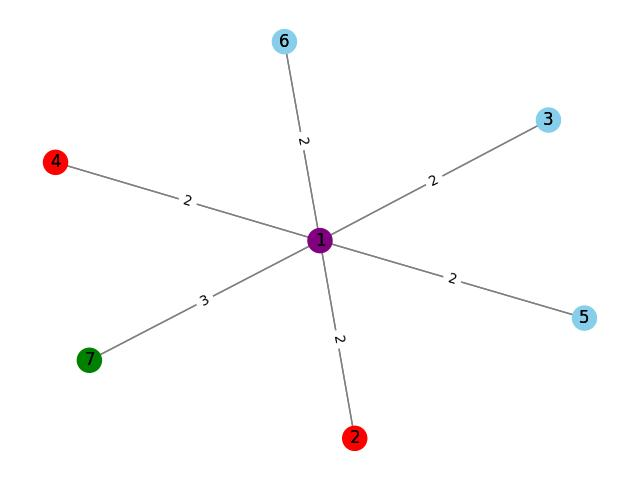
\includegraphics[width=1\linewidth]{2.jpg}
    \label{fig:my_label}
\end{figure}


\begin{figure}
    \centering
    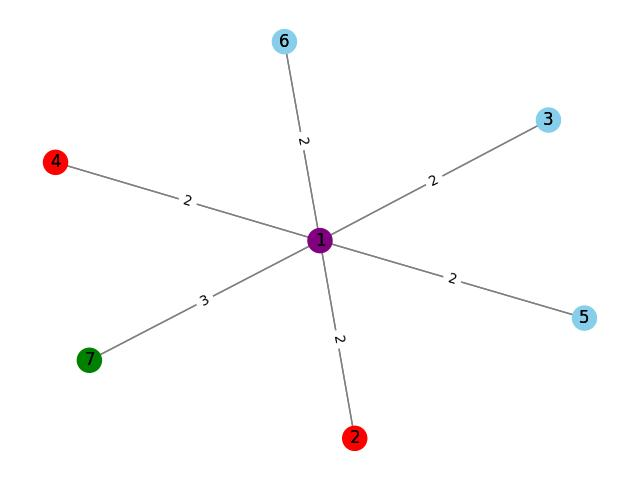
\includegraphics[width=1\linewidth]{2.jpg}
    \label{fig:enter-label}
\end{figure}

\begin{figure}
    \centering
    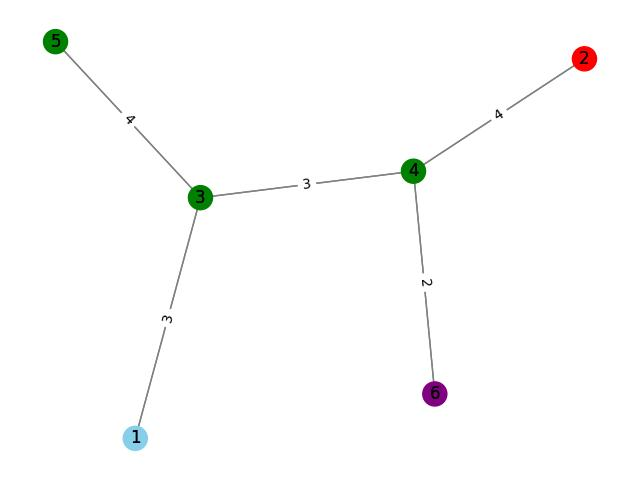
\includegraphics[width=1\linewidth]{3.jpg}
    \label{fig:enter-label}
\end{figure}

\begin{figure}
    \centering
    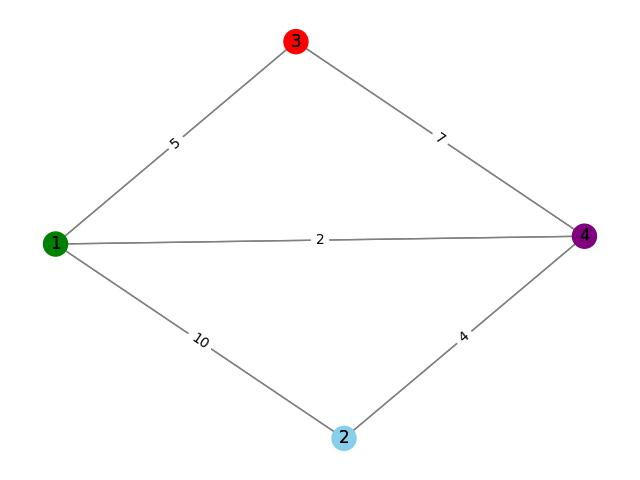
\includegraphics[width=1\linewidth]{4.jpg}
    \label{fig:enter-label}
\end{figure}

\begin{figure}
    \centering
    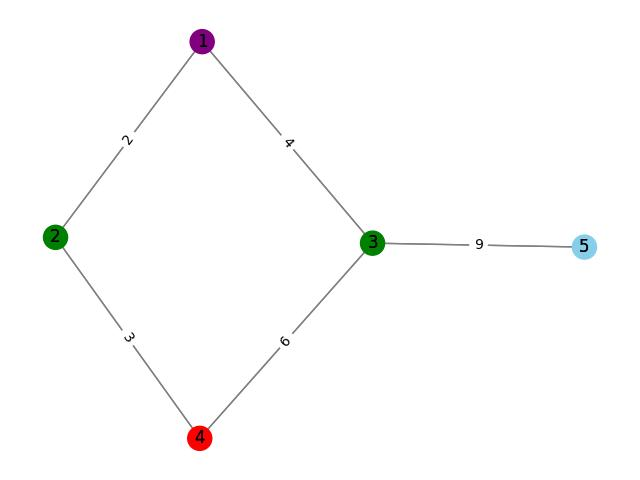
\includegraphics[width=1\linewidth]{5.jpg}
    \label{fig:enter-label}
\end{figure}

\begin{figure}
    \centering
    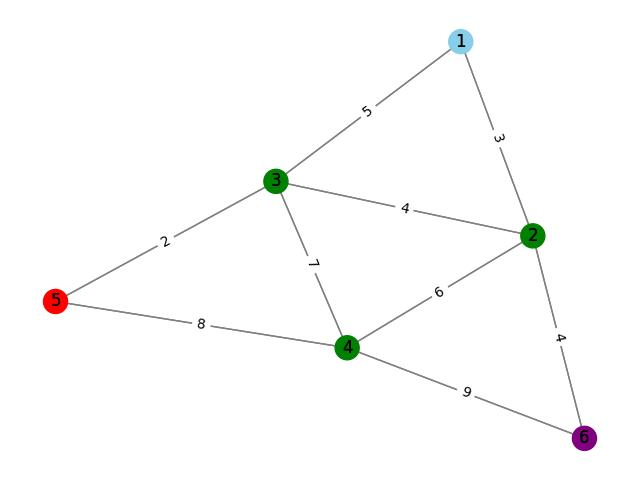
\includegraphics[width=1\linewidth]{6.jpg}
    \label{fig:enter-label}
\end{figure}

\begin{figure}
    \centering
    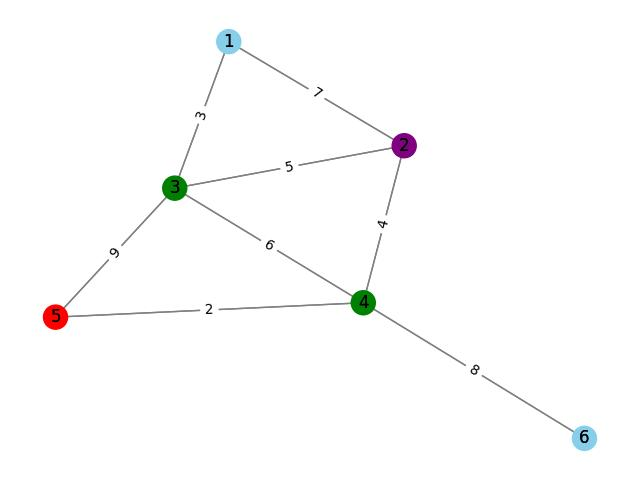
\includegraphics[width=1\linewidth]{7.jpg}
    \label{fig:enter-label}
\end{figure}

\begin{figure}
    \centering
    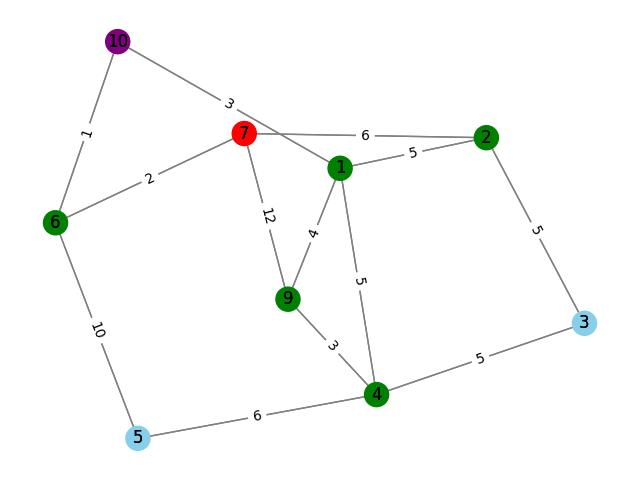
\includegraphics[width=1\linewidth]{8.jpg}
    \label{fig:enter-label}
\end{figure}

\begin{figure}
    \centering
    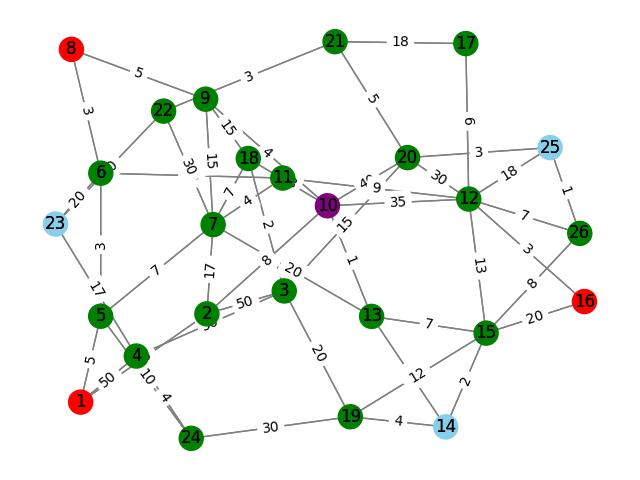
\includegraphics[width=1\linewidth]{9.jpg}
    \label{fig:enter-label}
\end{figure}

\clearpage

\section{Hipoteza  $H_1$}
\textbf{$H_1$:} Algorytm  $A_2$ zwykle daje dokładniejsze wyniki niż $A_1$. Różnica dokładności rośnie wraz z rozmiarem macierzy i liczbą niezerowych współczynników.

\hspace{}

\textbf{Wykresy różnicy $A_1$ - $A_2$}

\begin{figure}[ht!]
    \centering
    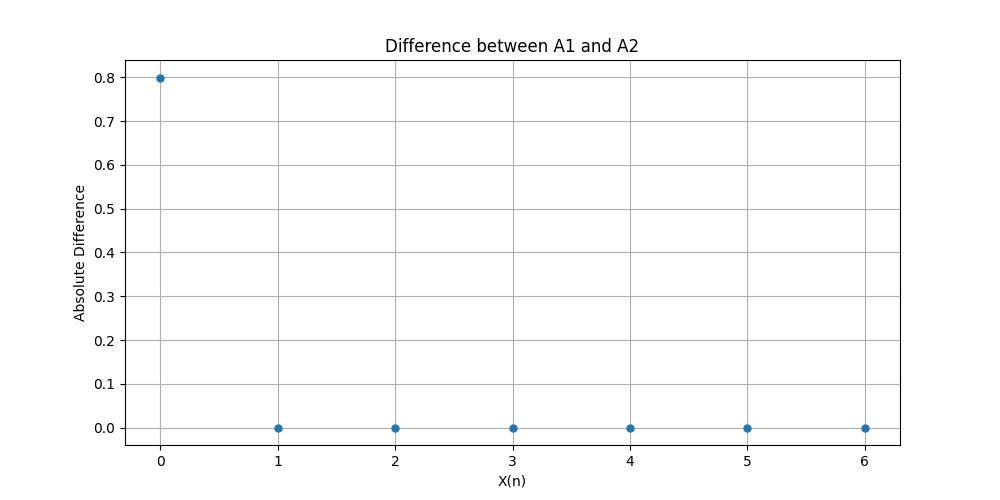
\includegraphics[width=1\linewidth]{h1_plot_1.jpg}
    \label{fig:my_label}
\end{figure}


\begin{figure}[ht!]
    \centering
    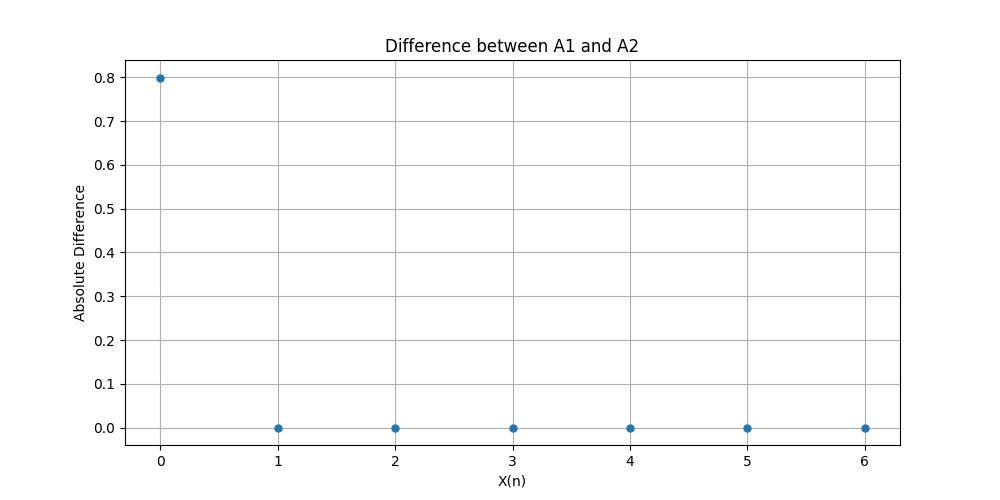
\includegraphics[width=1\linewidth]{h1_plot_2.jpg}
    \label{fig:enter-label}
\end{figure}

\begin{figure}
    \centering
    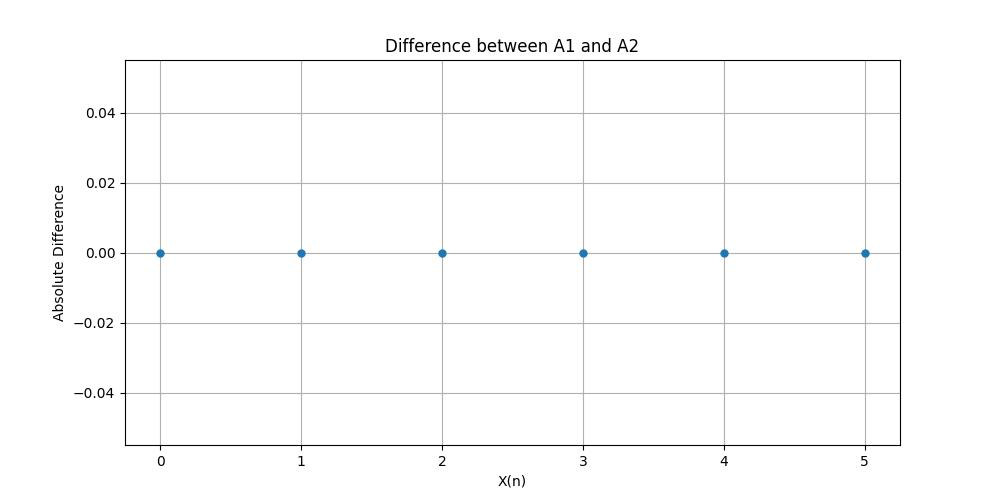
\includegraphics[width=1\linewidth]{h1_plot_3.jpg}
    \label{fig:enter-label}
\end{figure}

\begin{figure}
    \centering
    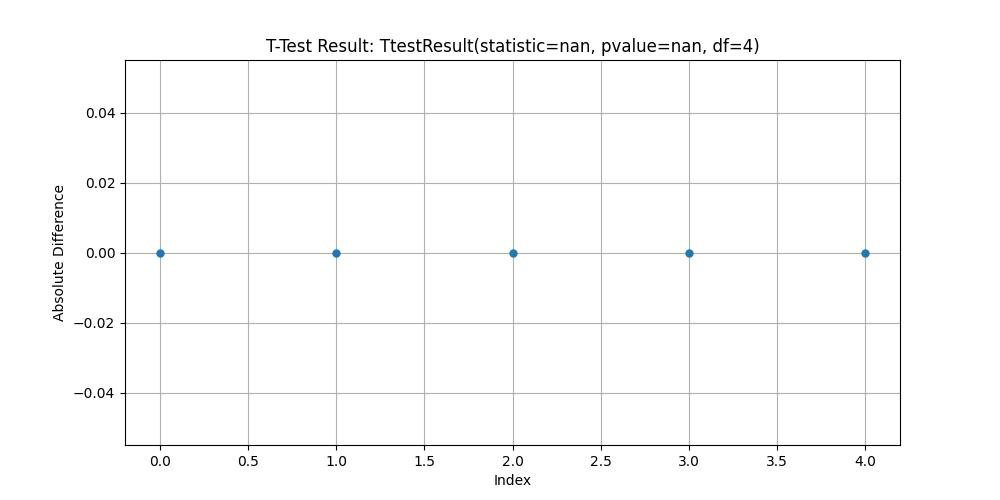
\includegraphics[width=1\linewidth]{h1_plot_4.jpg}
    \label{fig:enter-label}
\end{figure}

\begin{figure}
    \centering
    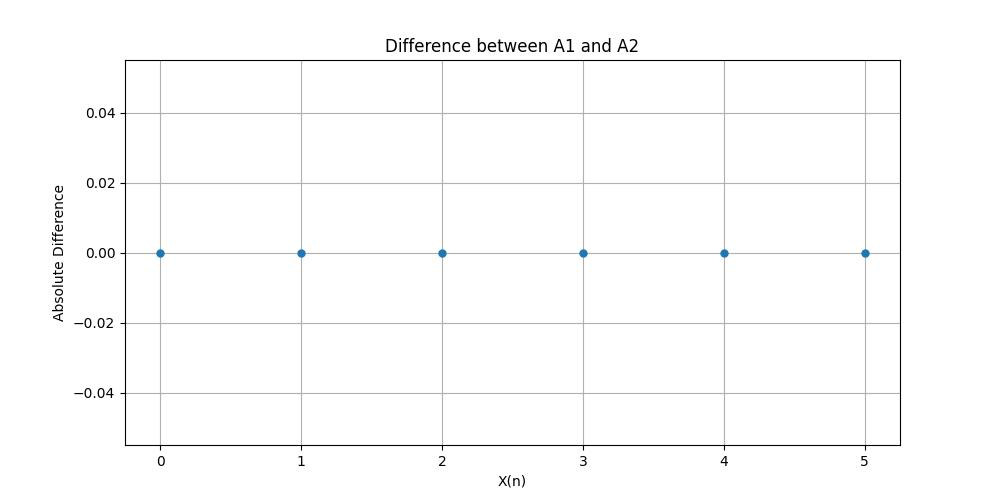
\includegraphics[width=1\linewidth]{h1_plot_5.jpg}
    \label{fig:enter-label}
\end{figure}

\begin{figure}
    \centering
    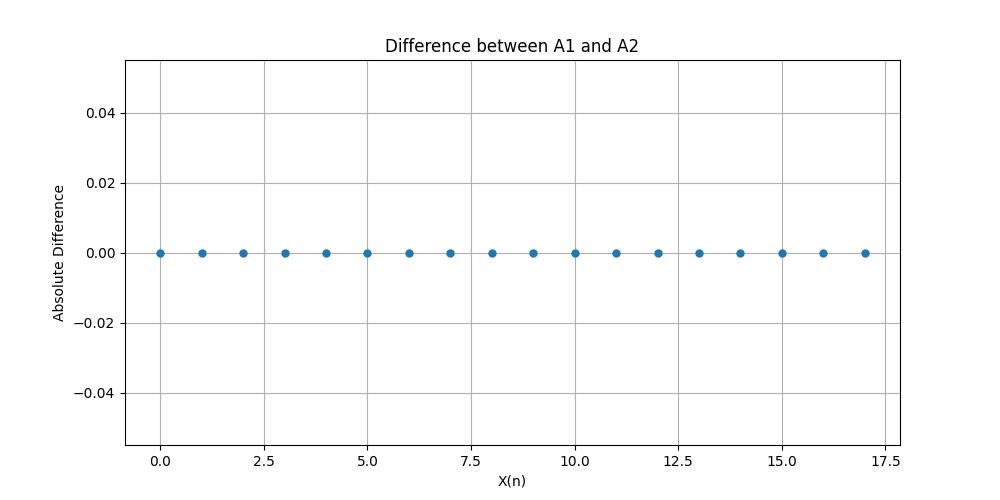
\includegraphics[width=1\linewidth]{h1_plot_6.jpg}
    \label{fig:enter-label}
\end{figure}

\begin{figure}
    \centering
    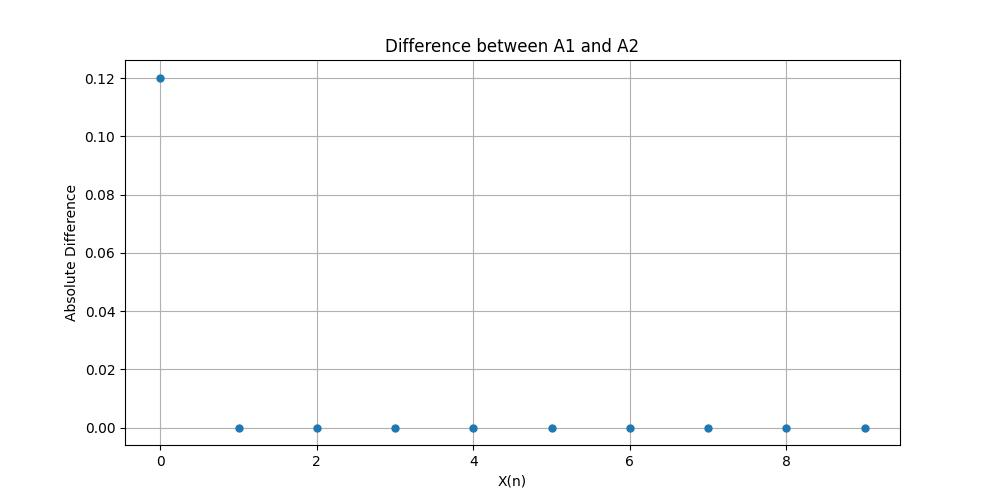
\includegraphics[width=1\linewidth]{h1_plot_7.jpg}
    \label{fig:enter-label}
\end{figure}

\begin{figure}
    \centering
    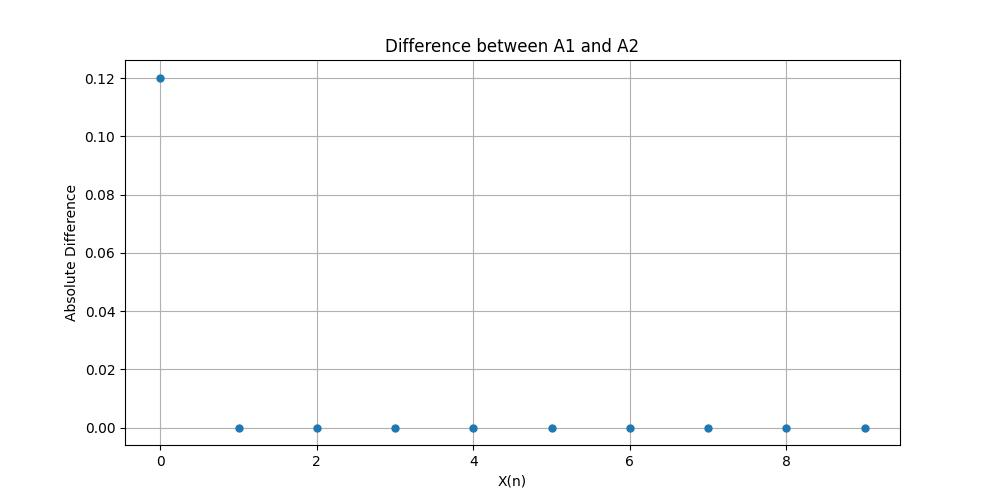
\includegraphics[width=1\linewidth]{h1_plot_8.jpg}
    \label{fig:enter-label}
\end{figure}

\begin{figure}
    \centering
    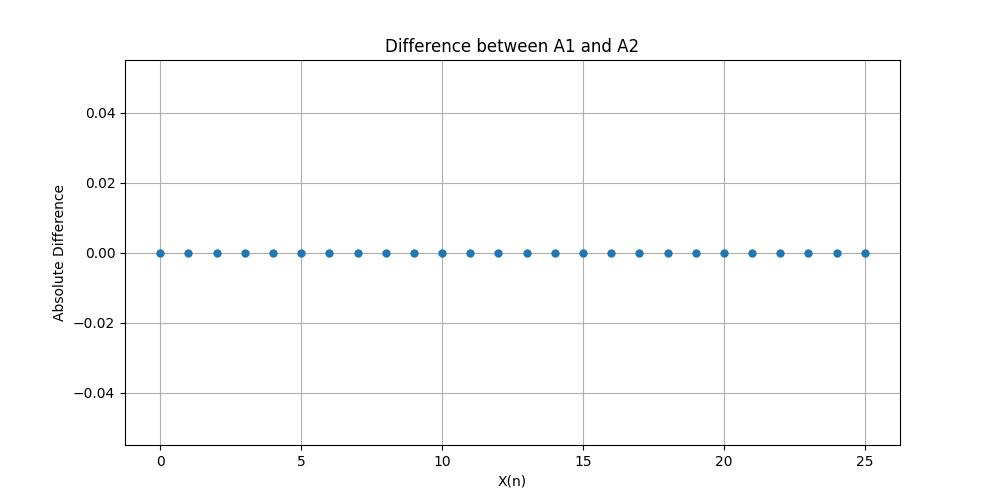
\includegraphics[width=1\linewidth]{h1_plot_9.jpg}
    \label{fig:enter-label}
\end{figure}



\textbf{Hipoteza nieprawdziwa.} 

\clearpage

\section{Hipoteza $H_2$}

\textbf{Algorytm $A_3$ działa dla postawionego zadania.}

\hspace{}

\textbf{Wykresy różnicy $A_1$ - $A_3$}

\begin{figure}[ht!]
    \centering
    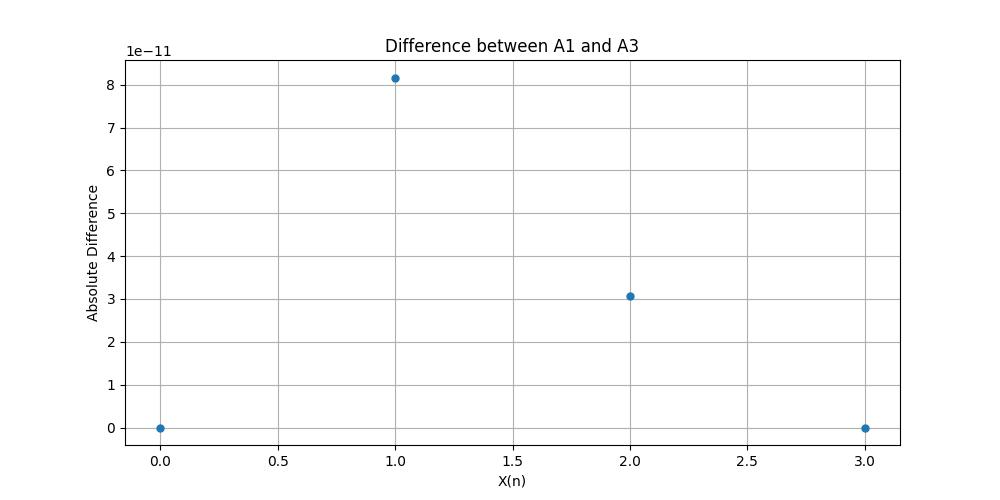
\includegraphics[width=1\linewidth]{h2_plot_1.jpg}
    \label{fig:my_label}
\end{figure}


\begin{figure}[ht!]
    \centering
    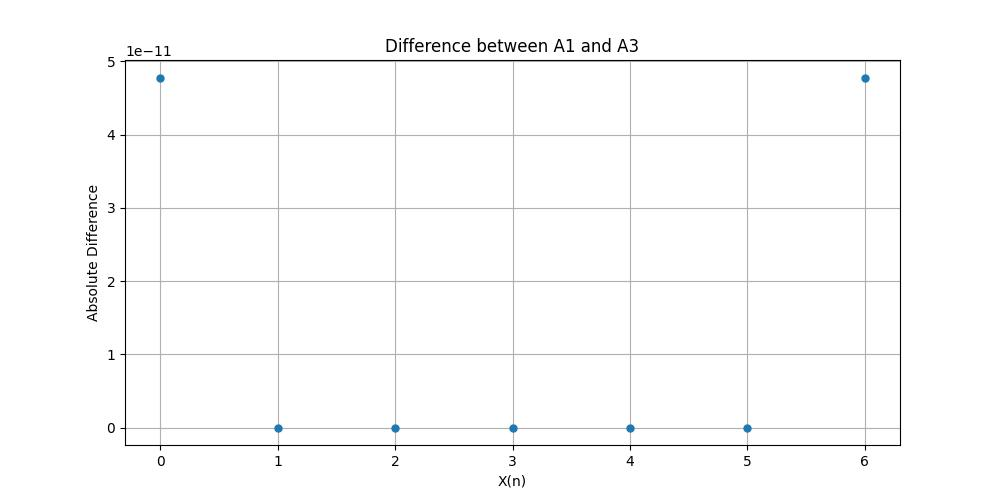
\includegraphics[width=1\linewidth]{h2_plot_2.jpg}
    \label{fig:enter-label}
\end{figure}

\begin{figure}
    \centering
    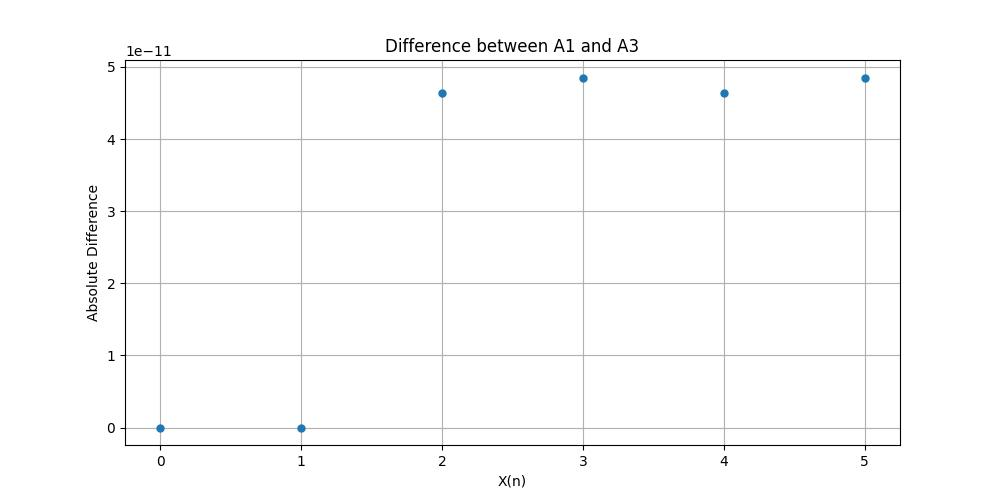
\includegraphics[width=1\linewidth]{h2_plot_3.jpg}
    \label{fig:enter-label}
\end{figure}

\begin{figure}
    \centering
    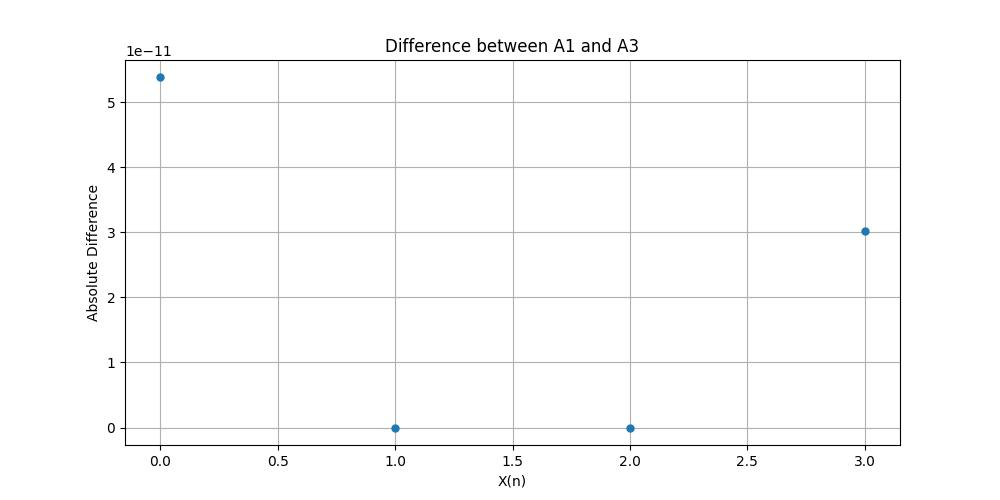
\includegraphics[width=1\linewidth]{h2_plot_4.jpg}
    \label{fig:enter-label}
\end{figure}

\begin{figure}
    \centering
    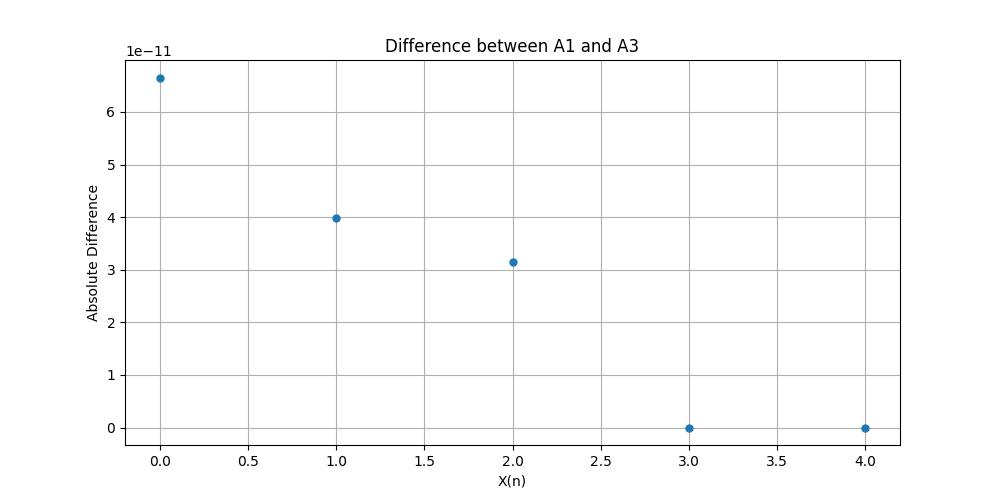
\includegraphics[width=1\linewidth]{h2_plot_5.jpg}
    \label{fig:enter-label}
\end{figure}

\begin{figure}
    \centering
    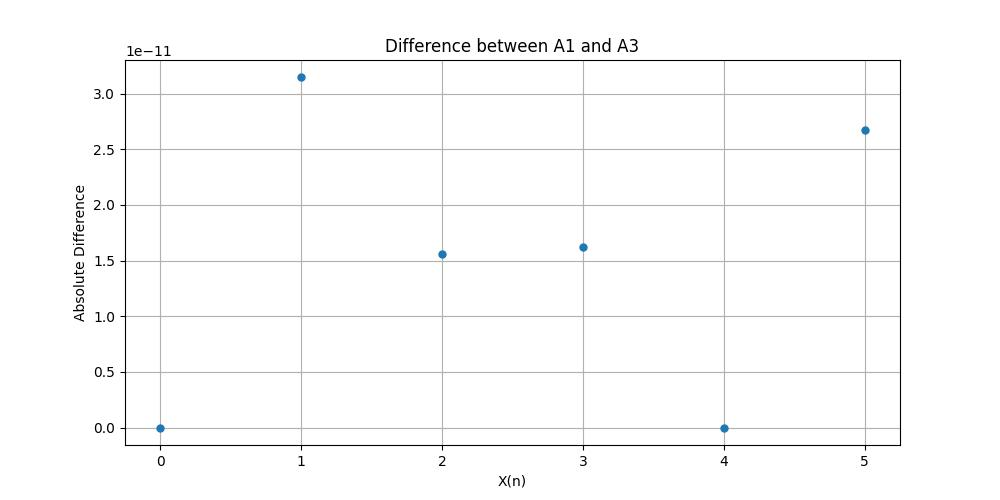
\includegraphics[width=1\linewidth]{h2_plot_6.jpg}
    \label{fig:enter-label}
\end{figure}

\begin{figure}
    \centering
    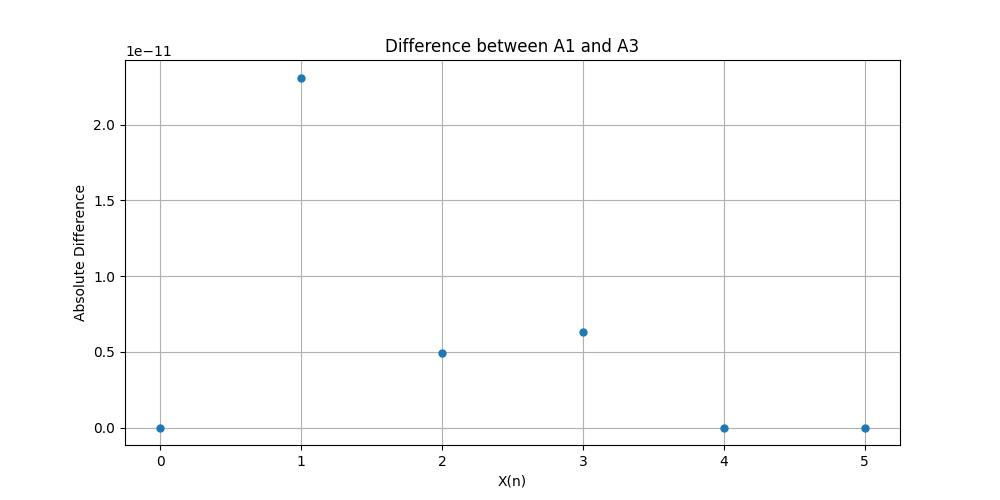
\includegraphics[width=1\linewidth]{h2_plot_7.jpg}
    \label{fig:enter-label}
\end{figure}

\begin{figure}
    \centering
    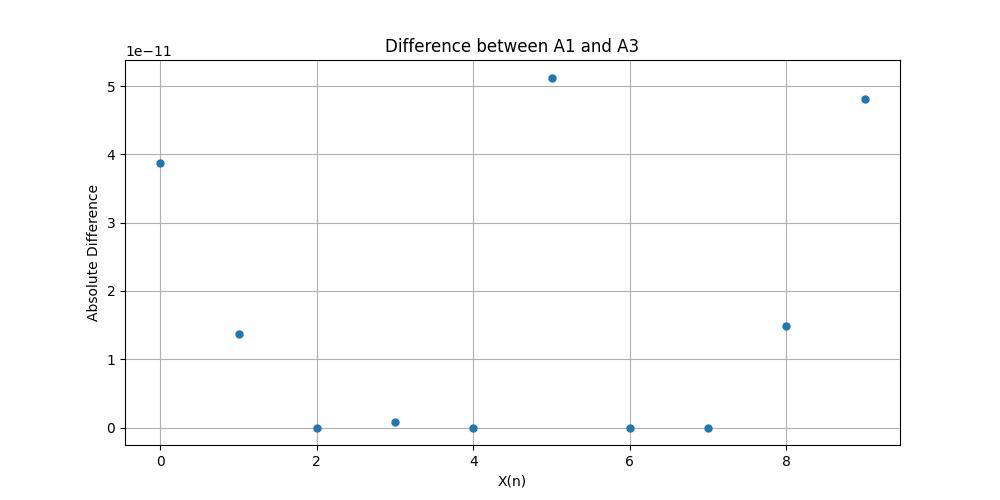
\includegraphics[width=1\linewidth]{h2_plot_8.jpg}
    \label{fig:enter-label}
\end{figure}

\begin{figure}
    \centering
    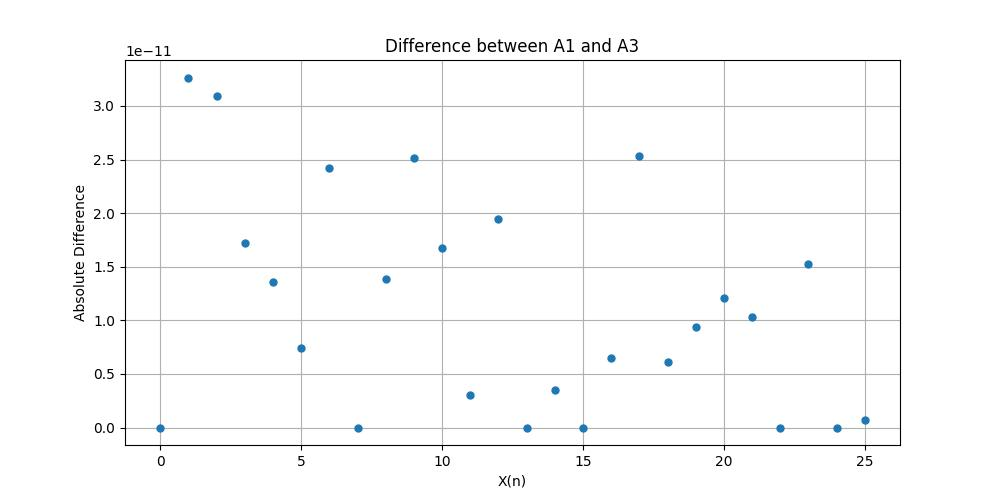
\includegraphics[width=1\linewidth]{h2_plot_9.jpg}
    \label{fig:enter-label}
\end{figure}



\textbf{Hipoteza prawdziwa. Róznica pomiędzy wynikami jest na oscyluje w granicy 1e-11 co przyjmujemy za dopuszczalne} 


\clearpage

\section{Hipoteza $h_3$}

\textbf{$H_3$: Jeśli algorytm $A_3$ jest zbieżny do rozwiązania, to wyniki otrzymujemy istotnie szybciej niż dla $A_1$ i $A_2$}

\begin{figure}[ht!]
    \centering
    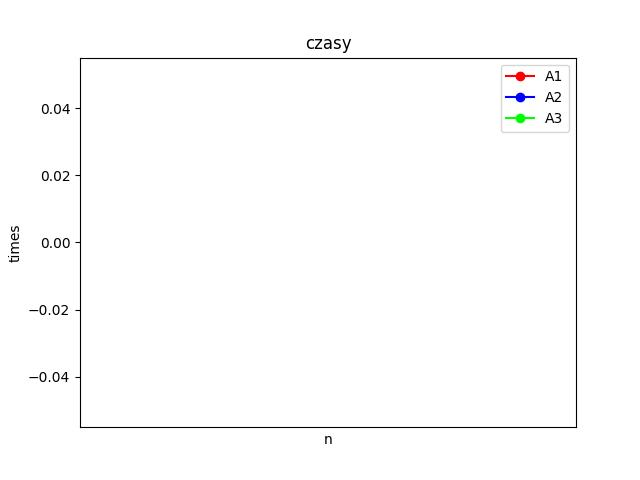
\includegraphics[width=1\linewidth]{czasy.jpg}
    \label{fig:enter-label}
\end{figure}



\textbf{Hipoteza nieprawdziwa.} 

\end{document}



